
\chapter{Background}\label{ch:background}

In this chapter, we provide the fundamental knowledge required to understand
the key concepts presented in our work.
At the very beginning, we strict formulate the problem definition.
Afterward, we present the process of transformation an audio sample to spectral input features,
which next are used as the input data to the \textit{Deep~Neural~Network} model.
Then in the section~\ref{sec:deep-neural-networks}, we introduce the key components
of \textit{Deep~Neural~Network}, where we focus on \textit{Recurrent~Neural~Networks} (\acrshort{rnn}),
and optimization techniques commonly used for RNNs.
At the end of the chapter, we present~\nameref{sec:connectionist-temporal-classification} algorithm,
which allows the \acrshort{rnn} models to be successfully used in automatic speech recognition systems.


\section{Problem Definition}\label{sec:problem-definition}

Let a single utterance $x^{(i)}$ and transcript $y^{(i)}$ be sampled from a training set defined as
$X=\{(x^{(1)}, y^{(1)}), (x^{(2)}, y^{(2)}), \ \dots\}$.
Each utterance $x^{(i)}$ is a time-series of length $T^{(i)}$, where every time-slice at $t$
is a vector of spectral input features $x_t^{(i)}$.
Each transcript $y^{(i)}$ is a sequence of characters present in the alphabet.

The goal of the model is to convert an input sequence $x^{(i)}$ into an output sequence $y^{(i)}$.
At each time-step $t$, the model returns probability distribution over each symbol in the alphabet
$\mathbb{P}(\ell | x^{(i)}_t)$.
In Polish we define an alphabet as $\ell \in \{ a, b, c \dots, \texit{space}, \texit{blank}\}$\footnote{
The used polish alphabet is composed of: \textit{a}, \textit{ą}, \textit{b}, \textit{c}, \textit{ć}, \textit{d}, \textit{e},
\textit{ę}, \textit{f}, \textit{g}, \textit{h}, \textit{i}, \textit{j}, \textit{k}, \textit{l}, \textit{ł}, \textit{m},
\textit{n}, \textit{ń}, \textit{o}, \textit{ó}, \textit{p}, \textit{r}, \textit{s}, \textit{ś}, \textit{t}, \textit{u},
\textit{w}, \textit{y}, \textit{z}, \textit{ź}, \textit{ż}, \textit{v}, \textit{x}, \textit{space}, \textit{blank}.
}, where we have added \textit{space} to denote word boundaries and \textit{blank} token due to the objective constrain.

The model output, a sequence of a probability distribution over each symbol in the alphabet, can be
decoded to a prediction $\hat{y}$ thanks to the \textit{CTC Inference} algorithm.
The model is trained using the \textit{CTC Loss} function, which measures prediction error.
Then we can backpropagate a gradient, update the parameters, and improve model performance.
Both the \textit{CTC Inference} and the \textit{CTC Loss} are presented in details in the
section~\nameref{sec:connectionist-temporal-classification}.


\section{Spectral Input Features}\label{sec:spectral-input-features}

In this section, we present how a \textit{continuous} speech signal is transformed to
the \textit{spectral input features}.
Therefore, we introduce the fundamental definitions in signal processing,
such as a signal representation in time and frequency domain, needed to understand our feature extraction process.
We start from defining the speech as a \textit{discrete} signal in the time domain.
For this purpose, we present two basic methods the \textit{sampling} and the \textit{quantization}.
Then, we transform a signal into the frequency domain and focus on the \textit{spectrogram}
as the short-time frequency analysis tool.
Based on a spectrogram, we define our spectral input feature representations, which are
\textit{Mel-scale~Log~Filter~Banks}.

The \textit{Mel-scale~Log~Filter~Banks} are the collection of filters scaled
according to the \textit{mel-scale}~\cite{stevens1937}.
The reason of use filter banks as input features is that the cochlea,
in the human ear, resembles a filter bank.
Additionally, the filter banks ranges are scaled using Mel-Scale which reflects
humans frequency perception.
Both the filter bank and the mel-scale tries to mirror humans speech perception.


\subsection*{Signal Representation in Time Domain}

Humans make speech sounds using speech organs such as the tongue, lips, and palate.
The result of this complex process is the \textit{sound pressure} change,
which is a variation of air pressure caused by a sound wave.
The amount of sound pressure change is measured by \textit{amplitude}.
A speech waveform is a representation of sound in the time domain, which shows changes of amplitude through time.
Speech is an analog signal, where the range and the domain of a signal are continuous.
Analog signals are hard to be processed on computers, so they need to be converted into
digital signals, of which domains and ranges are discrete.

To achieve a discrete domain, we have to measure the signal's value at specific points of interest.
This process is called as the \textit{uniform sampling}.
Let $x_a(t)$ be a continuous signal as a function of time $t$.
If we sample $x_a$ with a sampling period $T$, the output digital signal of this process is $x[n] = x_a(nT)$.
The \textit{sampling frequency} $F_s$ is defined as the inverse of the sampling period $F_s = 1/T$,
where its unit is hertz (Hz).

To achieve a discrete range, the continuous values of the signal have to be converted into a discrete set of values.
This process is called as the \textit{quantization}.
In an audio signal, the quantization level is defined as \textit{bits depth},
which represents the number of bits needed to represent the range of the signal.
For example, values of the 16-bit signal are in the range from -32768 to 32767.

Both processes the sampling and the quantization can cause the loss in signal information (additional noises).
The \textit{sampling~frequency} and the \textit{bit~depth} need to be high enough in order to achieve
a good approximation of the original continuous signal.
The main difficulty is to choose the right trade-off between the discrete signal quality and its size.


\subsection*{Pre-emphasis Audio Signal}
At the very beginning, we apply the pre-emphasis filter on the raw discrete audio signal to amplify the high frequencies.
The pre-emphasis is not a critical step, but it is useful to balance the frequency spectrum
since high frequencies usually have smaller magnitudes compared to lower frequencies.
The pre-emphasis filter is applied to a speech signal $x[n]$ as:
\begin{align}
y[n] = x[n] - \alpha \cdot x[n-1]
\end{align}
where $\alpha$ is common in the range from 0.95 to 0.97.


\subsection*{Signal Representation in Frequency Domain}

The \textit{Frequency domain} is a different perspective to look at a signal
besides the time domain.
Speech signal can be represented as a composition of
the \textit{pure} tones, which correspond specific frequencies.
The process of signal decomposition, changing a signal from the time domain to the frequency domain,
is called as the \textit{spectral transformation}.

Speech signals are non-stationary, which means that the statistical properties
of the signal change over time (intensity, variance, \ldots).
The speech signal can be considered as stationary and periodic in short time intervals.
Therefore we are able to analyze the \textit{short-time} intervals using the \textit{Fourier transformation}.
The short-time constraints lead us to a set of techniques called the \textit{Short-Time Analysis}.
The idea is to split a signal into short time frames (usually overlapped),
wherein we consider a signal in one frame as stationary, and then
transform each frame separately.
However, we have to be aware that frames should be short enough to satisfy assumptions, in practice, 10 to 40 ms.

Given the speech signal $x[n]$, the \textit{short-time signal} $x_m[n]$ of the frame $m$ is defined as:
\begin{align}
x_m [n] = x[n] \cdot w_m [n]
\end{align}
with $w_m[n]$ is the window function.
The window function is the same for all frames, so it can be simplified as:
\begin{align}
w_m [n] = w[m-n]
\end{align}
with $0 \leq n \leq N-1$, where $N$ is the frame length.
We assured the audio to be periodic by framing the signal.
Additionally, we apply the window function $w[n]$  on every frame to avoid
artifacts on window edges, and to reduce the signal discontinuity.
Therefore we can use the \textit{Hamming} function~\cite{harris1978}:
\begin{align}
w[n]=0.54-0.46 \cdot \cos(\frac{2 \pi n}{N-1})
\end{align}
Each frame $m$ of a signal is Fourier transformed, and the results are collected in the matrix,
which gathers the magnitude (a phase is usually neglected) for each point in time and frequency.
This can be expressed as:
\begin{align}
X(m, \omega)=\sum _{n=-\infty }^{\infty }x[n]w[n-m]e^{-j \omega n }
\end{align}
Then the spectrogram magnitude is computed as:
\begin{align}
S(m, \omega) = |X(m, \omega)^{2}|
\end{align}

The spectrograms can be the \textit{wide-band} and the \textit{narrow-band} depend on the window length.
Wide-band spectrograms use a short window length (<10 ms) which corresponds to
filters with a wide bandwidth (>200 Hz).
In opposite, narrow-band spectrograms use a longer window (>20 ms) which
leads to narrow bandwidth (<100 Hz).
In consequence, two kinds of spectrograms differ in time and frequency representation.
Wide-band spectrograms have a good \textit{time resolution}, so they are able to track pitches precisely.
In contrast, narrow-band spectrograms give a good view of the \textit{frequency resolution}.
Nevertheless, rapid changes over time are harder to distinguished.


\subsection*{Mel-scale Log Filter Banks}

The filter-banks is the collection of filters, which are spread out over audible frequencies,
and measure the energy amount within the part of the signal spectrum.
The mel spaced filter-banks are an attempt to reflect closely the human perception~\cite{stevens1937}.
The mel is a unit of ”measure of perceived pitch or frequency of a tone”.
In 1940, Stevens and Volkman assigned 1000 mels as 1000 Hz, and asked participants to change
the frequency until they perceived the pitch
changed some proportions with regard to the reference.
The threshold frequencies were marked, resulting in the mapping between
the real frequency scale (in Hz) and the perceived frequency scale (in mel).
The popular formula to convert from the frequency scale to the mel scale is:
\begin{align}
f_{mel} = 1125 \: \ln (1 + \frac{f_{Hz}}{700}).
\end{align}
where $f_{mel}$ is the frequency in mels and $f_{Hz}$ is the frequency in Hz.
According to the mel scale, humans are more sensitive to lower frequencies (figure~\ref{fig:mel_scale} on the left).

\begin{figure}[!h]
    \centering
    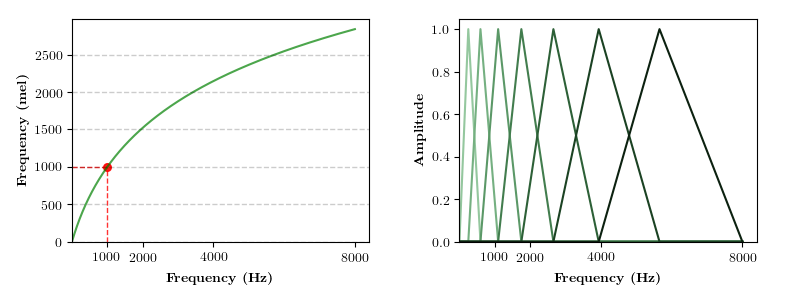
\includegraphics[width=13cm]{figures/mel-scale.png}
    \caption{
    The relationship between the frequency scale and mel scale is shown on the left.
    The Mel-scale filter-bank composed of 7 filters is presented on the right.
    }
    \label{fig:mel_scale}
\end{figure}

The mel-scale filter-banks contains $M$ filters, where the number of filters
defines the output resolution.
Each filter has a triangular shape and is spaced uniformly on the mel scale.
The filter functions are defined as:
\begin{align}
H_m(k) =
  \begin{cases}
      \hfill 0                                      \hfill & k < f(m - 1)                   \\[10pt]
      \hfill \dfrac{k - f(m - 1)}{f(m) - f(m - 1)}  \hfill & f(m - 1) \leq k < f(m)         \\[10pt]
      \hfill 1                                      \hfill & k = f(m)                       \\[10pt]
      \hfill \dfrac{f(m + 1) - k}{f(m + 1) - f(m)}  \hfill & f(m) < k \leq f(m + 1)         \\[10pt]
      \hfill 0                                      \hfill & k > f(m + 1)
  \end{cases}
\end{align}
where $H_m$ denotes the magnitude of the filter $m$, the frequency is denoted by $k$ and the vector $f$
contains $M+2$ linearly spaced filter border values (figure~\ref{fig:mel_scale} on the right).
To sum up, the mel-filter banks is composed of the high filter resolution
where human hearing is precise and the low resolution where it is inaccurate.
At the end of the feature extraction process, we use the logarithm to enhance signal details, which
leads to the \textit{Mel-scale~Log~Filter~Banks} representation.


\section{Deep Neural Networks}\label{sec:deep-neural-networks}

Our models are entirely based on the \textit{Deep~Neural~Networks} (\acrshort{dnn}), which are
used for the function approximation.
The \acrshort{dnn} is a stack of hidden layers, computational nodes which are differentiable.
Our models are composed of many standard building blocks like the linear layer, the convolutional layer, and
several nonlinear function such as the logistic sigmoid function ($\operatorname{sigmoid}$), the
hyperbolic tangent function ($\tanh$) or the rectified nonlinear unit ($\operatorname{relu}$).
In this section we briefly introduce the \textit{Recurrent~Neural~Networks} (\acrshort{rnn})
and optimization techniques which are common for the \acrshort{rnn}.
Other more novel or sophisticated building blocks such as the \acrshort{lstm}
are introduced in the section where they are used.


\subsection*{Recurrent Neural Networks}

To use an arbitrary amount of temporal context, what is crucial in speech recognition, we use the
\textit{Recurrent~Neural~Networks} (\acrshort{rnn}).
The \acrshort{rnn} build the hidden representation $h_t$ in time $t$
based on the current input $x_t$, and the previous hidden state $h_{t-1}$:
\begin{align}
h_t = f(x_t, h_{t-1}).
\end{align}
A vanilla RNN model $f$ is defined as:
\begin{align}
    h_t = g(W x_t + U h_{t-1} + b)
\end{align}
where $g$ is a nonlinearity function such as the rectified nonlinear unit ($\operatorname{relu}$).
The weights $W$, $U$, and $b$ are trainable parameters.
Moreover, the \acrshort{rnn} can be the \textit{bidirectional}, where past $h_{t-1}$
and future $h_{t+1}$ information is taken into account in building representation $h_t$.
The equations for the bidirectional \acrshort{rnn} are:
\begin{align}
    \overrightarrow{h}_t &= f(x_t, \overrightarrow{h}_{t-1}) \\
    \overleftarrow{h}_t &= f(x_t, \overleftarrow{h}_{t-1})   \\
    h_t &= \overrightarrow{h}_t + \overleftarrow{h}_t
\end{align}
In this case, we sum the forward and backward hidden states, but also a common
practice is to concatenate them.


\subsection*{Optimization}

In our work, we use a variation of the \textit{Stochastic~Gradient~Descent} (\acrshort{sgd})
to optimize the model's parameters.
The method is called the stochastic because it uses randomly selected samples to evaluate
the gradients, hence the \acrshort{sgd} can be regarded as a stochastic approximation of
gradient descent optimization.
The basic \acrshort{sgd} update is given by:
\begin{align}
    \theta_{t} = \theta_{t-1} - \eta_t \nabla_{\theta} \mathcal{L}(X, Y)
\end{align}
where $\mathcal{L}(X, Y)$ is the loss function computed on the training pair
$(X, Y)$ and $\eta_t$ is the \textit{learning rate} used at time $t$.
The \textit{mini-batch} is commonly used due to computationally constrains.
Moreover, it can reduce fluctuations, as the gradient computed at each step
is averaged over more training examples.

The \textit{momentum} augments the plain \acrshort{sgd} algorithm with a velocity term and can
accelerate learning (an analogy to momentum in physics):
\begin{align}
    v_t &= \rho v_{t-1} + \eta_t \nabla_{\theta} \mathcal{L}(X, Y) \\
    \theta_t &= \theta_{t-1} - v_t
\end{align}
Here the parameter $\rho$ dictates the amount of momentum to use and is
typically in the range $[0.9, 0.99]$.
Unlike in classical stochastic gradient descent, it tends to keep traveling in
the same direction, preventing oscillations.

There are vast alternative methods which attempt to blend estimations
of the first or second-order information of the gradient.
They try to approximate the \textit{Hessian} information, which is in practice hard to achieve.
In our work, we use the \textit{Adaptive~Moment~Estimation}~\cite{kingma2014}, which running averages of both the gradients,
and the second moments of the gradients.
Adam's parameter update is given by:
\begin{align}
    & m_{w}^{(t+1)} \leftarrow \beta_{1} m_{w}^{(t)}+(1-\beta_{1})\nabla_{w}L^{(t)}               \\[5pt]
    & v_{w}^{(t+1)}\leftarrow \beta _{2} v_{w}^{(t)}+(1-\beta_{2})(\nabla_{w}L^{(t)})^{2}         \\[5pt]
    & \hat{m}_w = \frac {m_{w}^{(t+1)}}{1-(\beta_{1})^{t+1}}                                      \\[5pt]
    & \hat{v}_w = \frac {v_{w}^{(t+1)}}{1-(\beta_{2})^{t+1}}                                      \\[5pt]
    & w^{(t+1)} \leftarrow w^{(t)} - \eta \frac{\hat{m}_w}{\sqrt{\hat{v}_w}+\epsilon}
\end{align}
where $\epsilon$ is a small scalar used to prevent division by 0, and $\beta_1$ and $\beta _{2}$
are the forgetting factors for gradients and second moments of gradients, respectively.
Squaring and square-rooting are done elementwise.
With $(\beta_1)^{t+1}$~and~$(\beta_2)^{t+1}$ we denote $\beta_1$~and~$\beta_2$ to the power~$t+1$.


\section{Connectionist Temporal Classification}\label{sec:connectionist-temporal-classification}

The dataset contains pairs of spectral input features $x^{(i)}$ and corresponding transcript $y^{(i)}$, but
we do not know how transcript aligns to the input.
To hand-align each character to its location is indeed time-consuming.
The attempts of hand-drafted rule-based approaches fail,
because both length and ratio of length vary between each sequence $x^{(i)}$~and~$y^{(i)}$.
In consequence, we can not directly use the supervised classification algorithms.
The \textit{Connectionist~Temporal~Classification} (\acrshort{ctc}) is the way
to overcome the lack of alignment between the input and the output~\cite{graves2006}.
The model for a sequence $x^{(i)}$ returns a sequence of distribution over all possible elements,
which can appear in $y^{(i)}$.
The \acrshort{ctc} algorithm use this distributions either to assess the \textit{probability} of a correct output
(\textit{Loss~Function}) or to \textit{infer} a most probable output (\textit{Inference}).
In both cases, they use the key concept of the \textit{Alignment}, which we briefly presented at the
beginning of this section.
Then we introduce the \textit{Loss~Function} and the \textit{Inference} algorithms as the crucial parts of
each \acrshort{ctc} based \acrshort{asr} system.
We encourage to check the \acrshort{ctc} in-depth analysis presented in~\cite{hannun2017}, especially
to distinguish a connection to other architectures such as \textit{encoder-decoder}.


\subsection{Alignment}\label{subsec:alignment}

The sequence of allowed elements, which can appear in $y^{(i)}$, forms the \textit{alignment}.
The \acrshort{ctc} appends the special \textit{blank} token to the alphabet.
Using the \textit{blank} token, we address two issues.
Firstly, it does not make sense to force a model to predict a character when nothing is there.
Secondly, it enables to predict repeated characters in a row.

% valid alignments figure (concatenate three of them)

The model returns the vast number of alignments, but only some of them are valid.
The valid alignments is a set of alignments which collapse (\textit{marginalize}) to the same output.
The \acrshort{ctc} marginalizes alignments in two steps.
It merges repeated elements and then removes \textit{blank} tokens.
Finally, summing the probability of valid alignments, the \acrshort{ctc} can estimate the output probability,
which is used either to calculate the \textit{loss} or to do \textit{inference}.

Worth to sum up the fundamental properties of \acrshort{ctc} alignments.
The alignments between $x^{(i)}$ and $y^{(i)}$ are monotonic and in a relation many-to-one, what
implies a third property that the length of $y^{(i)}$ cannot be greater than the length of $x^{(i)}$.


\subsection{Loss Function}\label{subsec:loss-function}

The \textit{CTC~Loss~Function} $\mathcal{L}$ for a single $(X, Y)$ pair is defined as:
\begin{align}
& \mathbb{P}(Y \mid X) \ = \sum_{A \in \mathcal{A}_{X,Y}} \prod_{t=1}^T \ p_t(a_t \mid X)      \\[5pt]
& \mathcal{L}_{CTC}(X, Y) = -\log \ \mathbb{P}(Y \mid X)
\end{align}
where $\mathcal{A}_{X,Y}$ describes valid alignments.
The model's parameters are tuned to minimize the negative log-likelihood.
The \acrshort{ctc} conditional probability marginalizes over the set of valid alignments
computing the probability for a single alignment step-by-step.
The straightforward approach scoring each alignment and sum them up fails due to
the massive number of alignments.
Thanks to the dynamic programming algorithm, we can efficiently compute the loss function.
The crucial insight is that two alignments can be merged if they have reached the same
output at the same time~\cite{hannun2017}.

The \textit{CTC~Loss} is fully differentiable with respect to the prediction at each time step,
since the objective just sums the product of them.
In result, it is possible to compute the gradient, and run the backpropagation as usual.


\subsection{Inference}\label{subsec:inference}

After the model training, we want to find the most probable output $\hat{Y}$ for a given input $X$,
what can be described as:
\begin{align}
  \hat{Y} \ = \ \underset{Y}{\operatorname{argmax}} \ p(Y \mid X)
\end{align}
To have in mind fact that a single output can have many alignments,
we have to use the beam search.
A regular beam search at each time step generates the new set of hypothesis, which
extends the previous hypothesis with all possible characters, and
then it keeps only the most probable candidates.
The beam search can be modified to store the output prefixes solely
after a marginalize process~\cite{hannun2017}.
